\section{Model Optimization}
\label{sec:optimizerStrategies}

When analyzing the range of values obtainable by a model, frequently a key question is ``what set of
parameters result in the best response value?''  To answer this question, RAVEN uses the \xmlNode{Optimizer},
a powerful sampler-like entity that searches the input space to find minimum or maximum values of a response.

In the remainder of this section, we will explore how to use the optimizer using a simple analytic problem,
with a two-dimensional input space and single response of interest.  After getting used to running with the
optimizer, we will add increasing complexity, including changing adaptive step sizes, initial conditions,
parallel trajectories, input space subdivision, input space constraints, and response constraints.

To demonstrate the operation of the Optimizer entities in RAVEN, the model we consider is the Beale function,
which is documented in the analytic tests for RAVEN and replicated here:

\begin{itemize}
  \item Function: $f(x,y) = (1.5-x+xy)^2+(2.25-x+xy^2)^2+(2.625-x+xy^3)^2$
  \item Domain: $-4.5 \leq x,y \leq 4.5$
  \item Global Minimum: $f(3,0.5)=0$
\end{itemize}

The two inputs are the variables $x$ and $y$, and the response is a value we'll assign to $ans$, short for
``answer''.  The model is an external model in RAVEN, and can be found at
\begin{verbatim}
  raven/tests/framework/AnalyticModes/optimizing/beale.py.
\end{verbatim}
The function's values are distributed as in Fig. \ref{fig:beale}.
\begin{figure}[h!]
  \centering
  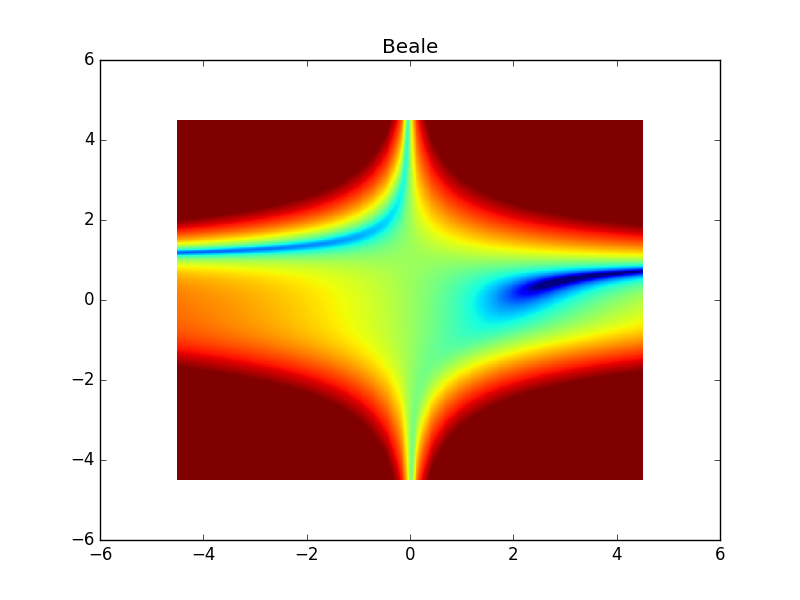
\includegraphics[scale=0.7]{../../tests/framework/user_guide/optimizing/Beale_grid.png}
  \caption{Plot of Beale's function for Optimization}
  \label{fig:beale}
\end{figure}

Note that throughout this example we use the SPSA optimizer by way of demonstration, since it is the first
advanced algorithm for optimization included in RAVEN; many of the options and parameters apply to other
optimizers, and details can be found in the RAVEN user manual.

\subsection{Introduction: The Optimizer Input}
As with other entities, the Optimizer gets its own XML block in the RAVEN input.
Here's an example of an input for a SPSA optimizer named \xmlString{opter}:
\xmlExample{framework/user_guide/optimizing/simple.xml}{Optimizers}
This is the smallest amount of input needed to run an optimization problem, with the exception that we include
the \xmlNode{initialSeed} to maintain consistent results.  Note the required blocks included
to define the optimizer:
\begin{itemize}
  \item \xmlNode{TargetEvaluation}, which declares the DataObject that the optimization search evaluations are
    going to be placed in.  All of the optimal points found as part of the optimization, as well as any other
    points evaluated as part of the algorithm, are placed in this object so the optimizer can retrieve this
    information later.  When this data object is defined, it is critical that the objective variable is
    defined in the output space, and the input variables in the input space, so the optimizer can collect the
    results of its sampling.  The data object type should be ``PointSet'' for this data object.  In this
    example, we use the self-descriptive \emph{optOut} data object.
  \item \xmlNode{variable}, which is where you can define the input space variables, one for each of these
    nodes.  Declaring a variable here informs the optimizer that you want it to find the optimal value for
    this variable, along with the other variables declared in their own blocks.  Additionally, you define the
    upper and lower bounds of the variable, which will give the optimizer some general expectations for
    finding the optimal point; it will never try to sample a value smaller than the lower bound or larger than
    the upper bound.  In the example we define variables \emph{x} and \emph{y} as our input variables, and
    both of them coincidentally range between -4.5 and 4.5.  We set the initial values for both variables to 0
    through the \xmlNode{initial} block, which is required in most cases; the exception is when a
    preconditioner sets them in mulitlevel optimization, but we're not concerned with that feature at this
    point.
  \item \xmlNode{objectVar}, which is where you indicate the variable for which you want to find the minimum (or,
    if you change the default, maximum).  As listed here, we want to minimize the value of \emph{ans} given a
    range of possible values for {x} and {y}.
\end{itemize}
The other critical blocks in this input are as follows:

\subsubsection{Models}
\xmlExample{framework/user_guide/optimizing/simple.xml}{Models}
Note that we define the external model with the name \xmlString{beale} and provide a path to the analytic
model itself.  This model is set up with the \texttt{run} method that allows RAVEN to run the model.  We also
list all our input/output variables, \emph{x, y}, and \emph{ans}.

\subsubsection{Data Objects}
\xmlExample{framework/user_guide/optimizing/simple.xml}{DataObjects}
We have three data objects: \xmlString{dummyIN}, which is necessary to define the input space of our external
model in the Steps; \xmlString{optOut}, which will hold all of the samples taken by our optimizer; and
\xmlString{opt\_export}, which will hold the actual solution path taken by our optimizer.  Note that while
\xmlString{optOut} is a Point Set, \xmlString{opt\_export} is a History Set.  This is because we store the
path travelled by the optimization algorithm as a history, with \emph{varsUpdate} keeping track of the
optimization steps taken.  Note especially how the input of \xmlString{opt\_export} is set to \emph{trajID},
which is a special keyword for the Optimizer history tracking, as is the output variable \emph{varsUpdate}.
There are several other special keyword outputs that can be written to the Solution Export data object, that
can be found in the user manual.

\subsubsection{Out Streams}
\xmlExample{framework/user_guide/optimizing/simple.xml}{OutStreams}
Here we define the way to print the output of our optimization algorithm.  There's not much to note, except
that we'll be printing the optimization path as a History-based CSV.

\subsubsection{Steps}
\xmlExample{framework/user_guide/optimizing/simple.xml}{Steps}
Here we put it all together into a work flow that RAVEN can follow.  We only need two steps: one to optimize,
and one to print out the results.  To actually perform the optimization, we need a MultiRun step, which we
cleverly name \xmlString{optimize}.  For input we take the placeholder data object \emph{dummyIN}, which sets
up the input space of the model we defined, \emph{beal}.  Where a \xmlNode{Sampler} would normally go, we
include the \xmlNode{Optimizer} we defined earlier.  We output to the same data object we indicated in the
Optimizer's \xmlNode{TargetEvaluation} node.  Finally, we note specifically the use of the
\xmlNode{SolutionExport} node.  The data object defined in this node is where the Optimizer will write the
optimization path history, with the final entry being the last step taken by the optimizer.  The IOStep is
unremarkable, used simply to write out the optimization path history to file.

\subsubsection{Conclusion}
After reviewing the components (don't forget the RunInfo block!), you can run this example and see the
results.  In particular, we can view the history of the optimizer in \texttt{Simple/opt\_export\_0.csv}.  Note
that \texttt{opt\_export} is the name of the \xmlNode{Print} OutStream we defined in the input file, and the
\texttt{\_0} indicates this is the first optimization path followed (we'll cover multiple paths later in
section \ref{subsec:opt parallel traj}).

When we open the file (preferably in a CSV reader such a spreadsheet viewer), we see a CSV with four headers,
the outputs defined in the data object in the input
file: \emph{x}, \emph{y}, \emph{ans}, and \emph{varsUpdate} (not necessarily in that order).  \emph{x},
\emph{y}, and \emph{ans} are the values of the variable at each optimization iteration, while
\emph{varsUpdate} gives the sequential order of the optimization iteration.

If we look at the last line, we converged around $f(1.61, -0.189) = 1.67$, which is okay but still quite a
ways from the analytic optimal point $f(3, 0.5) = 0$.  If we look at the output from the run, we can look at
the last time RAVEN was ``Checking convergence for Trajectory 0''.  Below that statement, there are a series
of convergence criteria and their status.  We can see that the reason we converged at the end is the
\texttt{Relative Loss Diff}, which means the relative change in the response \emph{ans} was sufficiently
small between steps to cause convergence.  Clearly, we claimed convergence prematurely because of the default convergence
values used by the optimizer.  Because these convergence criteria are very problem-specific, the default
parameters will not work best for all problems.

We can improve this result by changing convergence
parameters as well as step size growth and shrink factors, all of which can be found in the user manual, and
many of which we'll discuss in the rest of this section.

\subsection{Initial Conditions and Parallel Trajectories} \label{subsec:opt parallel traj}
Notice we set the optimization search to start at $(0,0)$.
%By default, RAVEN chooses the center
%point of the input space as an initial value.
You can change this initial value through
the \xmlNode{initial} block within the \xmlNode{variable} definition node.

Furthermore, RAVEN offers the possibility to run multiple optimization paths in parallel.  Because many
(perhaps most) optimization techniques get stuck in local minima, using multiple paths (or \emph{trajectories} as
they are called in RAVEN) increases the likelihood that one of the trajectories will find the global minimum
point.  You can request multiple trajectories by providing a variety of initial conditions in the
\xmlNode{initial} block, as shown in this Optimizer example:
\xmlExample{framework/user_guide/optimizing/multiple_trajectories.xml}{Optimizers}
Note that the ordered pairs are split across the \xmlNode{initial} nodes, so that the first trajectory will
start as a point made up of all the first entries, the second trajectory starts at all the second entries, and
et cetera.  In this case, we've requested starting points at (-2,-2), (-2,2), (2,-2), and (2,2).  This (and
defining a new working directory in the \xmlNode{RunInfo} block) is the only input change between the original
file and this one.

When run, we can see the results in the working directory \texttt{MultipleTraj}.  There, we see the same files
as for the base case, plus \texttt{opt\_export} files 0-3 instead of just 0.  Each of these corresponds to the
path that one of the initial points started at, as you can see at the top of each of these CSV files.  We can
see that trajectory 3 (who started at (2,2)) ended close to the analytic optimal point, while trajectory 0
was far from it.

In order to see a summary of the end point of each trajectory, we can use the additional RAVEN step described
in \ref{subsec:opt summarizing results}.


\subsection{Summarizing Results} \label{subsec:opt summarizing results}
While seeing the histories of the optimization paths taken in the \xmlNode{SolutionExport} is informative,
sometimes we just want to see the final optimal point found by each trajectory.  In this case, we can use an
\emph{InterfacedPostProcessor} called {HistorySetSnapShot} to get the last point found by each optimizer.  The
postprocessor looks like this:
\xmlExample{framework/user_guide/optimizing/summary.xml}{Models.PostProcessor}
Note that we named the postprocessor \xmlString{snapshot}, and instructed it to look for the \xmlString{max}
value of \xmlString{varsUpdate} in each of the histories, and combine them into a single data set.  We add the
following Step to our \xmlNode{Steps} to run it:
\xmlExample{framework/user_guide/optimizing/summary.xml}{Steps.PostProcess}
Don't forget to add \xmlString{getOptPoint} to the \xmlNode{Sequence} in the \xmlNode{RunInfo} block, before
\xmlString{print} but after \xmlString{optimize}.  Note that this post-processing step takes the
\xmlNode{SolutionExport} data object from the optimizing step as input, runs the postprocessing model, then
places the results in a new data object, \xmlString{opt\_soln}, which we add to the \xmlNode{DataObjects}
list in the input file.

Note also that we added the printing of the \xmlString{opt\_soln} data object to the \xmlString{print}
\xmlNode{IOStep}; we only needed to write an \xmlNode{OutStream} for it, not a whole new step.

After running this input, you can open \texttt{Summary/opt\_soln.csv} to see the final results of each
optimization trajectory.  The variable \emph{trajID} gives the trajectory label, \emph{x} and \emph{y} give
the final location of the optimal point found by that trajectory, \emph{ans} gives the value of the response
at that location, and \emph{varsUpdate} shows how many iterations were necessary to find that optimal point.
The trajectory with the lowest value for \emph{ans} is the most optimal point found.

\subsection{Adjusting Adaptive Steps} \label{subsec:opt stepsize}
As we've seen, some of the optimization paths are struggling to converge to meaningful optimal solutions.
One way to improve this is to tinker with the convergence tolerances defined in the user manual.  Another is
to change the step size modifications used as part of the search process, which we discuss in this section.
First, we briefly discuss how the SPSA chooses its step size, so we can make informed choices about what
parameters to use.

Because SPSA is a gradient-based method, it operates by starting at a particular point, estimating the
gradient at that point, then taking a step in the opposite direction of the gradient in order to follow a
downhill path.  It adaptively chooses how long of a step to take based on its history.  If the gradient is in
the same direction twice in a row, the algorithm assumes there's further to travel, so increases its step size
multiplicatively by the \emph{grainGrowthFactor}, which by default is 2.0 in RAVEN.  If, on the other hand,
the gradient switches directions, then the step size is divided by the \emph{gainShrinkFactor}, which again is
2.0 by default in RAVEN.  This means that by default, if the gradient keeps going in the same direction, you
always double your step size, while if you're bouncing back and forth in a valley, the step size is halved at
each iteration.

By way of note, in higher dimensions, the actual growth or shrink multiplier is scaled by a dot product
between the two previous gradients, with a max of the grain growth factor when the dot product is 1 (exactly
aligned) and a minimum of grain shrink factor when the dot product is -1 (exactly opposite).  This means if
the gradient is at right angles with the past gradient, then the step size remains unchanged (dot product is
0).

There are some additional considerations for the step size change, as well.  If the algorithm takes a step,
then discovers the new point has a worse response value than the point it's at, it will reject the new point,
re-evaluate the gradient, and flag the step size to be divided by the gain shrink factor.  Because of this, if
the gain shrink factor is too large, false convergence can be obtained when the algorithm struggles to find a
new downhill point to move to.  As a result, in practice it is often beneficial to have a gain shrink factor
that is smaller than the gain growth factor.

For this particular example, we use gain growth factor of 1.5 (meaning when the gradient continues in the same
direction our step grows to 150\% of its old value) and a gain shrink factor of 1.25 (meaning when the
gradient flips directions our step size shrinks to 80\% of its old value).  We add this to the base case
(\texttt{simple.xml}) to get:
\xmlExample{framework/user_guide/optimizing/step_size.xml}{Optimizers}
Note the definition of the gain growth and shrink factors in the \xmlNode{convergence} block.  Reviewing the
output file \texttt{StepSize}, we can see more steps were taken than the case using default step sizes, but
the final solution was $f(2.65,0.403)=0.0286$, which is much closer to the analytical solution of $f(3,0.5)=0$
than the base case and within our convergence tolerances of the right solution.

It is often challenging to find the best gain growth and shrink factors, and these can have a very significant
impact on the speed and accuracy of the convergence process.  Too large a shrink factor results in poor
resolution of valleys, while too small a shrink factor results in many unnecessary evaluations of the model.

\subsection{Denoising Stochastic Problems}
While many of the models we see in optimization are deterministic (meaning running the same inputs into the
model yields the same results every time), there are quite a few stochastic models that we might desire to
optimize.  For example, a model that included Brownian motion or is solved using unseeded random numbers might
be considered stochastic.

The difficulty with optimizing noisy problems rests in the unreliability of a single sample.  If we send a
single set of inputs into a stochastic model, we can't trust the results to be consistent.  One way to measure
the consistency of the results is through a signal-to-noise ratio (SNR).  There are many ways to define this
value; for our purposes, we will use the ratio of the mean of the signal to the standard deviation of the
signal, $\mu/\sigma$.

To obtain an approximation of your SNR, you can use RAVEN to perform a Monte Carlo run on your model and then
use the BasicStatistics postprocessor to collect the mean (expectedValue) and standard deviation (sigma) of
your response.  It's important to make this sampling all at a single value in the input space, so replace your
variables with constants in the Sampler input.  Once you have the mean and sigma, you have an idea of how
noisy your model is.  A SNR of 1 means the signal is just as big as the noise, making it very difficult to
optimize.  A SNR of less than 1 means the noise dominates the signal, and will make optimization almost
impossible without introducing denoising.  A SNR of more than 1 indicates the signal is stronger than the
noise, and perhaps denoising is not necessary.  If your standard deviation is 0, then you don't have any
discernable noise!

To denoise a model in RAVEN SPSA optimization currently, we turn our attention to the \xmlNode{Optimizer}
subnode \xmlNode{parameter}, specifically the \xmlNode{numGradAvgIterations} node.  This parameter instructs
RAVEN to perform multiple gradient evaluations, including multiple evaluations of each optimal point, and use
the average to make decisions in optimization pathing.  By default, RAVEN takes one optimal point and one
neighboring point to evaluate a gradient.  Increasing the \xmlNode{numGradAvgIterations} will increase the
number of times the optimal point is sampled, and how many neighbor points are sampled.  This serves to
denoise the model.

However, this also raises the question, how many resamples do I need to denoise my model?  In a Wilks-like
approach, we want to reduce the size of the confidence interval for our mean to be less than the noise.  The
number of resamples required depends on the size of the confidence interval $z$ and the confidence-to-noise ratio
$\xi$ we want to ultimately have for the optimization algorithm.  We also assume the distribution of the
response is roughly Gaussian Normal, which may not be the case.  The approximate equation for assuring the
confidence interval is smaller than the noise is
\begin{equation}
  \frac{z\sigma}{\sqrt{n}} \leq \xi\sigma,
\end{equation}
\begin{equation}
  n \geq \left(\frac{z}{\xi}\right)^2.
\end{equation}
Thus, the number of resamples depends on the confidence level as well as the desired ratio of the confidence interval
to the noise.

A few values for varying ratios are given in Table \ref{tab:confidence levels} for the 99\% confidence level ($z=2.576$).
\begin{table}[htb]
  \centering
  \begin{tabular}{c c}
    Confidence-to-noise $\xi$ & Resamples necessary \\ \hline
    1.0 & 7 \\
    0.9 & 9 \\
    0.7 & 14 \\
    0.5 & 27 \\
    0.1 & 664 \\
    0.05 & 2655
  \end{tabular}
  \caption{Estimate of the number of samples necessary to denoise models to varying confidence levels}
  \label{tab:confidence levels}
\end{table}
That is, if you want the noise and confidence interval to have the same magnitude, only 7 resamples are
required.  If, on the other hand, you want the confidence interval to be half the level of the noise, 27
resamples are required.

Note these are only guidelines; individual models may behave differently and require more or less resamples to
provide a clear optimization path.

\subsection{Input Space Subdivision}
In higher-dimensional problems, sometimes the input space can be divided into characteristic subspaces.  For
example, potentially one set of inputs vary slowly with consistent gradient directions in the response, while
for another set of inputs the response fluctuates frequently with many local minima.  In this case, it might
be beneficial to optimize the subspaces in nested loops, slowly converging the smoothly-varying space while
often converging the undulating space.

For these cases, RAVEN provides \emph{multilevel} operation.  To transition our base case to a multilevel
case, we change the optimizer as follows:
\xmlExample{framework/user_guide/optimizing/multilevel.xml}{Optimizers}
Note the addition of the \xmlNode{multilevel} node.  In this node, we need to define the subspaces, then the
ordering of the subspaces in terms of convergence priority.  We intuitively name the subspace with \emph{x}
the \emph{xgroup} and similarly with \emph{y}.  Note that while in this example each subspace consists of only
one variable, in general many variables may exist in any given subspace.  Note also that it's a bad idea to
include a variable in multiple subspaces.

The \xmlNode{sequence} can be thought of as an order of nesting optimization, where the first subspace listed
is optimized most slowly (but only once) and the last is optimized frequently and swiftly.  Each time a new
optimal point is found, the innermost space (in our example \emph{yspace}) is converged completely, holding all
the variables in all other subspaces (e.g. \emph{xspace}) constant at their most recent value.  Once
\emph{yspace} is converged, we take a single step in the subspace \emph{xgroup}, then return to converging
\emph{yspace} again.  Every step in \emph{xspace} triggers a full convergence of \emph{yspace}.

In the results in \texttt{Multilevel/opt\_export\_0.csv}, you can observe how first one dimension then the
other is perturbed in the search for the optimal point.

It should be noted as well, using multilevel optimization does not necessarily improve the optimization path;
in fact, in many cases, the number of model evaluations increases significantly for little gain in final
optimal value.  Multilevel is most useful when clustered subspaces share a particular feature in optimization
that is useful to isolate from the rest of the optimization procedure, or if some subsets of inputs act
independently from others in affecting the response.


\subsection{Functional Constraints} \label{subsec:opt explicit constraint}
Sometimes an optimization problem has a constrained input space, possibly where there is a tradeoff between
two inputs.  In this event, RAVEN allows the user to define a \emph{constraint} function, which will cause
RAVEN to treat this constraint as it would a boundary condition.

For example, we will introduce a void in the input where we reject inputs.  This void is defined by rejecting
all samples within $(x-1)^2 + y^2 < 1$.  We'll also include the modified step growth and shrink parameters
discussed in section \ref{subsec:opt stepsize}.

To include a constraint function, we first have to define it in the RAVEN input as a \xmlNode{Function}
entity:
\xmlExample{framework/user_guide/optimizing/constrain.xml}{Functions}
Note that the file \texttt{./Constrain/constraint.py} is located relative to the working directory.  Currently,
external functions are always Python files.  In that file,
note that the only method is \texttt{constrain}, which is RAVEN's keyword to find the constraint function.
RAVEN will pass in a \texttt{self} object, which will have the function variables defined in the
\xmlNode{Functions} input available as members.  The method \texttt{constrain} then returns a boolean which is \texttt{True} if
the evaluation does not violate the constraint, or \texttt{False} if the constraint is violated.

To attach the constraint to the optimizer, simply add it as an assembled \xmlNode{Function}:
\xmlExample{framework/user_guide/optimizing/constrain.xml}{Optimizers}

After running, looking through the path followed by trajectory 0 shows that instead of following the path from
section \ref{subsec:opt stepsize}, the path moves to lower \emph{y} values before swinging back up toward the
optimal point.

%\subsection{Implicit Constraints (Penalties)}
% TODO come up with a working example
